% Three-colouring gadgets (generated by figs_c3ch09.py).
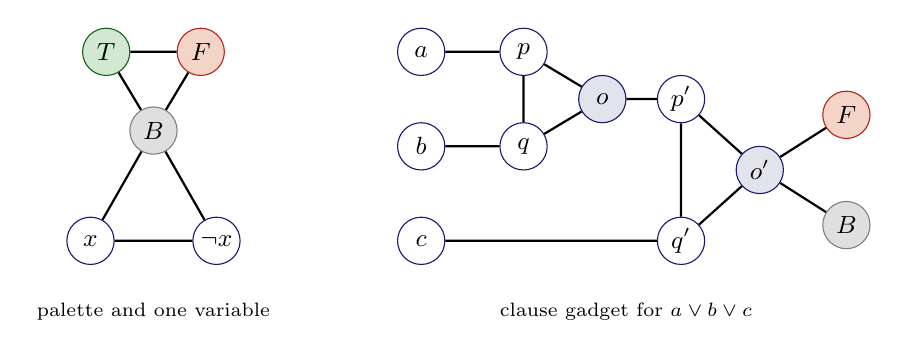
\begin{tikzpicture}[x=10mm,y=10mm,every node/.style={font=\small},
  v/.style={circle,draw=MidnightBlue,fill=white,minimum size=6mm,inner sep=0pt},
  t/.style={circle,draw=ForestGreen!70!black,fill=ForestGreen!20,minimum size=6mm,inner sep=0pt},
  f/.style={circle,draw=BrickRed,fill=BrickRed!15,minimum size=6mm,inner sep=0pt},
  b/.style={circle,draw=gray,fill=gray!25,minimum size=6mm,inner sep=0pt}]
\node[t] (T) at (0,1.6) {$T$};
\node[f] (F) at (1.2,1.6) {$F$};
\node[b] (B) at (0.6,0.6) {$B$};
\draw[thick] (T) -- (F) -- (B) -- (T);
\node[v] (x) at (-0.2,-0.8) {$x$};
\node[v] (nx) at (1.4,-0.8) {$\neg x$};
\draw[thick] (x) -- (nx) (x) -- (B) (nx) -- (B);
\node[font=\scriptsize,align=center] at (0.6,-1.7) {palette and one variable};
\node[v] (a) at (4.0,1.6) {$a$};
\node[v] (bb) at (4.0,0.4) {$b$};
\node[v] (c) at (4.0,-0.8) {$c$};
\node[v] (p1) at (5.3,1.6) {$p$};
\node[v] (q1) at (5.3,0.4) {$q$};
\node[v,fill=MidnightBlue!12] (o1) at (6.3,1.0) {$o$};
\node[v] (p2) at (7.3,1.0) {$p'$};
\node[v] (q2) at (7.3,-0.8) {$q'$};
\node[v,fill=MidnightBlue!12] (o2) at (8.3,0.1) {$o'$};
\node[f] (F2) at (9.4,0.8) {$F$};
\node[b] (B2) at (9.4,-0.6) {$B$};
\draw[thick] (a) -- (p1) (bb) -- (q1) (p1) -- (q1) -- (o1) -- (p1);
\draw[thick] (o1) -- (p2) (c) -- (q2) (p2) -- (q2) -- (o2) -- (p2);
\draw[thick] (o2) -- (F2) (o2) -- (B2);
\node[font=\scriptsize,align=center] at (6.6,-1.7) {clause gadget for $a\lor b\lor c$};
\end{tikzpicture}
